\documentclass[tikz,border=8pt]{standalone}
% Shared pastel academic grammar for final-size technical-paper diagrams.
\usepackage[T1]{fontenc}
\usepackage{lmodern}
\usepackage{amsmath,amssymb}
\usepackage{xcolor}
\usepackage{tikz}
\usetikzlibrary{
  arrows.meta,
  backgrounds,
  calc,
  circuits.logic.US,
  decorations.pathreplacing,
  fit,
  matrix,
  patterns,
  positioning,
  shapes.geometric,
  shapes.symbols
}

\definecolor{ink}{RGB}{24,24,28}
\definecolor{midink}{RGB}{96,96,104}
\definecolor{paleink}{RGB}{184,184,190}
\definecolor{wash}{RGB}{241,240,237}
\definecolor{paper}{RGB}{255,255,253}
\definecolor{cyan}{RGB}{126,203,218}
\definecolor{cyanwash}{RGB}{211,238,242}
\definecolor{pink}{RGB}{235,139,158}
\definecolor{pinkwash}{RGB}{250,211,217}
\definecolor{purple}{RGB}{166,50,150}
\definecolor{purplewash}{RGB}{232,196,227}
\definecolor{gold}{RGB}{177,139,45}
\definecolor{goldwash}{RGB}{239,226,183}
\definecolor{slate}{RGB}{116,133,145}
\definecolor{slatewash}{RGB}{221,226,229}
\colorlet{muted}{midink}
\colorlet{rule}{paleink}
\colorlet{accent}{purple}
\colorlet{accentwash}{purplewash}
\colorlet{second}{cyan}
\colorlet{secondwash}{cyanwash}

\tikzset{
  every picture/.style={
    font=\rmfamily\footnotesize,
    text=ink,
    line cap=round,
    line join=round,
    >=Stealth
  },
  every node/.style={outer sep=0pt},
  panel mark/.style={font=\rmfamily\bfseries\footnotesize},
  primary/.style={font=\rmfamily\footnotesize},
  secondary/.style={font=\rmfamily\scriptsize,text=midink},
  signal name/.style={font=\ttfamily\footnotesize,anchor=east},
  scope trace/.style={draw=ink,line width=.62pt,line cap=butt,line join=miter},
  hairline/.style={draw=paleink,line width=.28pt,line cap=butt},
  dotted guide/.style={draw=midink,line width=.32pt,densely dotted},
  dashed scope/.style={draw=ink,line width=.45pt,dashed},
  transition/.style={-{Stealth[length=1.8mm,width=1.25mm]},draw=ink,line width=.58pt},
  transition label/.style={font=\rmfamily\scriptsize,fill=paper,inner sep=1.2pt},
  preedge/.style={circle,draw=ink,fill=paper,line width=.58pt,minimum size=8.2mm,inner sep=1pt},
  observed preedge/.style={preedge,fill=purplewash,double,double distance=1.15pt,line width=.62pt,minimum size=9.8mm},
  brace/.style={decorate,decoration={brace,mirror,amplitude=3pt},draw=ink,line width=.45pt},
  grid rule/.style={draw=slate,line width=.32pt,line cap=butt},
  outer rule/.style={draw=ink,line width=.82pt,line cap=butt,line join=miter},
  star mark/.style={star,star points=5,star point ratio=2.2,draw=ink,fill=purple,minimum size=5.1mm,inner sep=0pt},
  % Compatibility vocabulary used by the repository's other figures.
  flow/.style={-{Latex[length=4.5pt,width=3.2pt]},draw=ink,line width=.55pt},
  heavy flow/.style={-{Latex[length=5pt,width=3.6pt]},draw=ink,line width=.8pt},
  wire/.style={draw=ink,line width=.5pt},
  bus/.style={draw=ink,line width=1.05pt},
  guide/.style={draw=midink,line width=.4pt,dotted},
  alternate/.style={draw=ink,line width=.5pt,dashed},
  scope/.style={draw=ink,line width=.5pt,dashed,inner sep=6pt},
  block/.style={draw=ink,line width=.55pt,fill=paper,minimum height=8mm,inner xsep=5pt,inner ysep=4pt,align=center},
  operation/.style={block,fill=cyanwash,minimum width=17mm},
  register/.style={block,fill=paper,minimum width=16mm,minimum height=10mm},
  state/.style={circle,draw=ink,line width=.55pt,fill=cyanwash,minimum size=8mm,inner sep=1pt,align=center},
  terminal/.style={state,fill=purplewash,double,double distance=1.2pt,line width=.6pt},
  predicate/.style={diamond,aspect=1.8,draw=ink,line width=.55pt,fill=pinkwash,inner xsep=3pt,inner ysep=2pt,align=center},
  datum/.style={rectangle,draw=ink,line width=.5pt,fill=goldwash,minimum width=8mm,minimum height=6mm,inner sep=2pt,align=center},
  panel label/.style={font=\rmfamily\bfseries\footnotesize},
  local heading/.style={font=\rmfamily\bfseries\footnotesize},
  annotation/.style={font=\rmfamily\scriptsize,text=midink,align=center},
  heading/.style={font=\rmfamily\bfseries\small},
  subheading/.style={font=\rmfamily\bfseries\footnotesize},
  note/.style={font=\rmfamily\scriptsize,text=midink},
  label/.style={font=\rmfamily\bfseries\scriptsize},
  mono/.style={font=\ttfamily\footnotesize},
  tiny mono/.style={font=\ttfamily\scriptsize},
  count/.style={font=\rmfamily\bfseries\small},
  selected/.style={draw=ink,fill=purplewash,line width=.8pt},
  cell on/.style={fill=purple,draw=ink,line width=.3pt},
  cell off/.style={fill=paper,draw=paleink,line width=.3pt}
}

% Flat pastel facets and depth edges for restrained axonometric constructions.
\tikzset{
  cyan facet/.style={draw=ink,fill=cyanwash,line width=.5pt,line join=round},
  cyan side/.style={draw=ink,fill=cyan,line width=.5pt,line join=round},
  pink facet/.style={draw=ink,fill=pinkwash,line width=.5pt,line join=round},
  pink side/.style={draw=ink,fill=pink,line width=.5pt,line join=round},
  purple facet/.style={draw=ink,fill=purplewash,line width=.55pt,line join=round},
  purple side/.style={draw=ink,fill=purple,line width=.55pt,line join=round},
  gold facet/.style={draw=ink,fill=goldwash,line width=.5pt,line join=round},
  gold side/.style={draw=ink,fill=gold,line width=.5pt,line join=round},
  context facet/.style={draw=ink,fill=slatewash,line width=.45pt,line join=round},
  depth edge/.style={draw=midink,line width=.38pt},
  surface grid/.style={draw=slate,line width=.32pt},
  projection/.style={draw=midink,line width=.38pt,densely dashed},
  accent curve/.style={draw=purple,line width=1.05pt},
  cyan curve/.style={draw=cyan!70!ink,line width=.9pt},
  pink curve/.style={draw=pink!70!ink,line width=.9pt},
  gold curve/.style={draw=gold!80!ink,line width=.9pt}
}


\tikzset{
  lane label/.style={
    font=\rmfamily\bfseries\footnotesize,
    anchor=west,
    fill=paper,
    inner xsep=1.4pt,
    inner ysep=.8pt
  },
  lane rule/.style={draw=rule,line width=.35pt},
  compact register/.style={register,minimum height=10mm,minimum width=25mm},
  code state/.style={state,minimum size=6.5mm,font=\ttfamily\scriptsize},
  stencil cell/.style={
    draw=ink,
    line width=.38pt,
    fill=paper,
    minimum width=6.3mm,
    minimum height=3.7mm,
    inner sep=.4pt,
    font=\rmfamily\scriptsize,
    align=center
  },
  current cell/.style={stencil cell,fill=purplewash,line width=.7pt},
  fact wire/.style={draw=purple!72!ink,line width=.58pt},
  x rail/.style={draw=cyan!65!ink,line width=1.05pt},
  position rail/.style={draw=gold!78!ink,line width=.9pt}
}

% A shallow stack reads as a bank of independent two-bit registers rather
% than as a single counter with a common overflow state.
\newcommand{\counterbank}[6]{%
  \path[draw=ink,fill=#6!65!paper,line width=.38pt]
    ({#2-1.27},{#3-.29}) rectangle ({#2+1.47},{#3+.49});
  \path[draw=ink,fill=#6!42!paper,line width=.42pt]
    ({#2-1.37},{#3-.39}) rectangle ({#2+1.37},{#3+.39});
  \node[register,fill=#6!20!paper,minimum width=28mm,minimum height=8mm]
    (#1) at (#2,#3) {\textbf{#4}\\[-1pt]\scriptsize #5};
}

\begin{document}
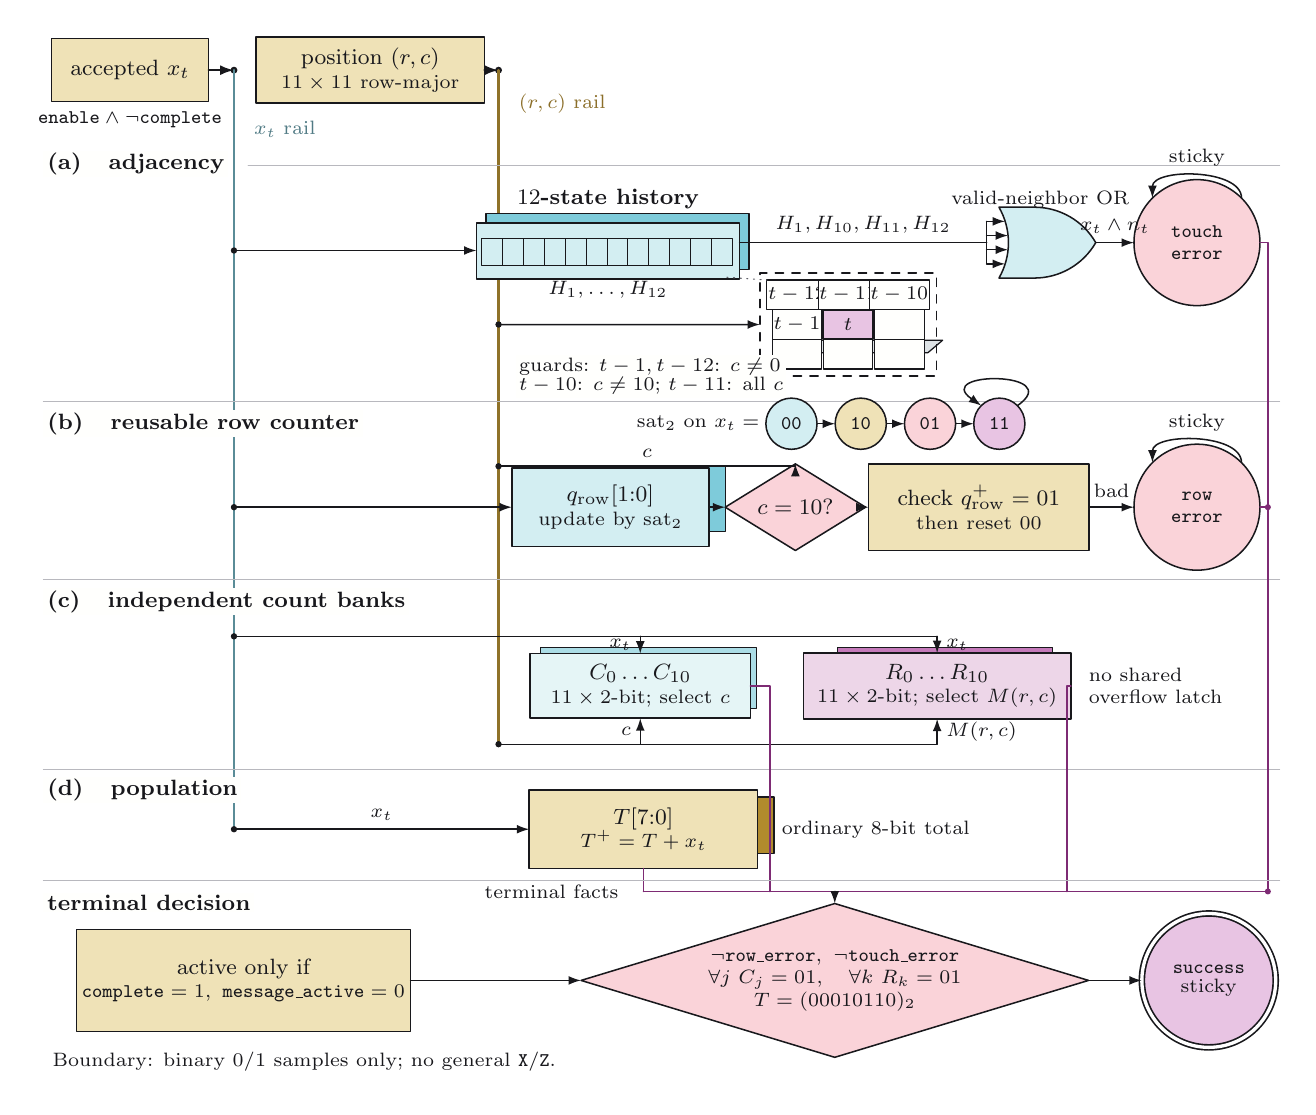
\begin{tikzpicture}[x=1cm,y=1cm]
  \path[use as bounding box] (0,0) rectangle (16,13.45);

  % The two top-level stream facts descend on separate, colored rails.
  \node[datum,minimum width=20mm,minimum height=8mm] (input) at (1.30,12.91)
    {accepted $x_t$};
  \coordinate (xtrunk) at (2.62,12.91);
  \draw[heavy flow] (input.east) -- (xtrunk);
  \fill[ink] (xtrunk) circle (1.25pt);
  \node[annotation,text=ink] at (1.30,12.28)
    {$\mathtt{enable}\land\neg\mathtt{complete}$};

  \node[register,fill=goldwash,minimum width=29mm,minimum height=8mm]
    (position) at (4.35,12.91)
    {position $(r,c)$\\[-1pt]\scriptsize $11\times11$ row-major};
  \coordinate (ptrunk) at (5.98,12.91);
  \draw[heavy flow] (position.east) -- (ptrunk);
  \fill[ink] (ptrunk) circle (1.25pt);
  \draw[x rail] (xtrunk) -- (2.62,3.27);
  \draw[position rail] (ptrunk) -- (5.98,4.35);
  \node[annotation,anchor=west,text=cyan!55!ink] at (2.76,12.16) {$x_t$ rail};
  \node[annotation,anchor=west,text=gold!75!ink] at (6.12,12.48) {$(r,c)$ rail};

  % Adjacency: a depth-stacked history tape projects onto a local stencil.
  \node[lane label] at (.20,11.72) {(a)\quad adjacency};
  \draw[lane rule] (2.80,11.70) -- (15.90,11.70);

  \path[cyan side] (5.82,10.38) rectangle (9.16,11.09);
  \path[cyan facet] (5.70,10.26) rectangle (9.04,10.97);
  \node[local heading] at (7.37,11.28) {$12$-state history};
  \foreach \k in {0,...,11} {
    \path[draw=ink,fill=cyanwash,line width=.27pt]
      ({5.76+.266*\k},10.43) rectangle ++(.266,.34);
  }
  \node[annotation,text=ink] at (7.37,10.12) {$H_1,\ldots,H_{12}$};
  \coordinate (history-west) at (5.70,10.62);
  \coordinate (history-east) at (9.04,10.72);
  \draw[flow] (2.62,10.62) -- (history-west);
  \fill[ink] (2.62,10.62) circle (1.15pt);

  % The slight offset beneath the stencil is a data plane, not another state.
  \path[context facet]
    (9.48,9.32) -- (11.43,9.32) -- (11.62,9.48) -- (9.67,9.48) -- cycle;
  \node[stencil cell] (ul) at (9.77,10.06) {$t-12$};
  \node[stencil cell] (up) at (10.42,10.06) {$t-11$};
  \node[stencil cell] (ur) at (11.07,10.06) {$t-10$};
  \node[stencil cell] (left) at (9.77,9.68) {$t-1$};
  \node[current cell] (cur) at (10.42,9.68) {$t$};
  \node[stencil cell] (mr) at (11.07,9.68) {};
  \node[stencil cell] (bl) at (9.77,9.30) {};
  \node[stencil cell] (down) at (10.42,9.30) {};
  \node[stencil cell] (br) at (11.07,9.30) {};
  \node[scope,fit=(ul)(ur)(bl)(br),inner sep=2.5pt] (stencil) {};
  \draw[guide] (8.88,10.28) -- (ul.north west);
  \draw[flow] (5.98,9.68) -- (stencil.west);
  \fill[ink] (5.98,9.68) circle (1.15pt);
  \node[annotation,anchor=west,align=left,text=ink,fill=paper,inner sep=1.2pt]
    at (6.20,9.02)
    {guards: $t-1,t-12$: $c\ne0$\\[-.4mm]
     $t-10$: $c\ne10$; $t-11$: all $c$};

  \node[or gate US,draw=ink,fill=cyanwash,line width=.55pt,
        logic gate inputs=nnnn,minimum size=9mm] (neighboror) at (12.86,10.72) {};
  \node[annotation,text=ink] at (12.86,11.27) {valid-neighbor OR};
  \coordinate (tapbus) at (12.18,10.72);
  \draw[wire] (history-east) -- node[annotation,above,text=ink]
    {$H_1,H_{10},H_{11},H_{12}$} (tapbus);
  \draw[wire] (tapbus |- neighboror.input 1) -- (tapbus |- neighboror.input 4);
  \foreach \i in {1,...,4} {
    \draw[flow] (tapbus |- neighboror.input \i) -- (neighboror.input \i);
  }
  \node[state,fill=pinkwash,minimum size=16mm,font=\rmfamily\scriptsize]
    (touch) at (14.85,10.72) {$\mathtt{touch}$\\$\mathtt{error}$};
  \draw[flow] (neighboror.output) -- node[annotation,above,text=ink]
    {$x_t\land n_t$} (touch.west);
  \draw[flow] (touch.north east) .. controls +(0,.38) and +(0,.38) ..
    node[annotation,above,text=ink] {sticky} (touch.north west);

  \draw[lane rule] (.20,8.70) -- (15.90,8.70);

  % The row counter is reused; the four states make the unusual encoding explicit.
  \node[lane label] at (.20,8.42) {(b)\quad reusable row counter};
  \node[annotation,anchor=west,text=ink] at (7.62,8.43)
    {$\operatorname{sat}_2$ on $x_t=1$:};
  \node[code state,fill=cyanwash] (s00) at (9.70,8.42) {00};
  \node[code state,fill=goldwash] (s10) at (10.58,8.42) {10};
  \node[code state,fill=pinkwash] (s01) at (11.46,8.42) {01};
  \node[code state,fill=purplewash] (s11) at (12.34,8.42) {11};
  \draw[flow] (s00) -- (s10);
  \draw[flow] (s10) -- (s01);
  \draw[flow] (s01) -- (s11);
  \draw[flow] (s11.north east) to[out=35,in=145,looseness=4.3] (s11.north west);

  \path[cyan side] (6.20,7.05) rectangle (8.86,7.89);
  \node[compact register,fill=cyanwash] (rowcount) at (7.40,7.36)
    {$q_{\rm row}[1{:}0]$\\[-1pt]\scriptsize update by $\operatorname{sat}_2$};
  \node[predicate,minimum width=15mm,minimum height=11mm] (endrow) at (9.75,7.36)
    {$c=10$?};
  \node[operation,fill=goldwash,minimum width=28mm,minimum height=11mm]
    (rowcheck) at (12.08,7.36)
    {check $q_{\rm row}^{+}=01$\\[-1pt]\scriptsize then reset $00$};
  \node[state,fill=pinkwash,minimum size=16mm,font=\rmfamily\scriptsize]
    (rowerror) at (14.85,7.36) {$\mathtt{row}$\\$\mathtt{error}$};
  \draw[flow] (2.62,7.36) -- (rowcount.west);
  \fill[ink] (2.62,7.36) circle (1.15pt);
  \draw[flow] (rowcount.east) -- (endrow.west);
  \draw[flow] (5.98,7.88) -| node[annotation,near start,above,text=ink] {$c$} (endrow.north);
  \fill[ink] (5.98,7.88) circle (1.15pt);
  \draw[flow] (endrow.east) -- (rowcheck.west);
  \draw[flow] (rowcheck.east) -- node[annotation,above,text=ink] {bad} (rowerror.west);
  \draw[flow] (rowerror.north east) .. controls +(0,.38) and +(0,.38) ..
    node[annotation,above,text=ink] {sticky} (rowerror.north west);

  \draw[lane rule] (.20,6.44) -- (15.90,6.44);

  % Persistent column and region counters are visibly separate stacks.
  \node[lane label] at (.20,6.16) {(c)\quad independent count banks};
  \counterbank{columns}{7.78}{5.09}{$C_0\ldots C_{10}$}{$11\times2$-bit; select $c$}{cyan}
  \counterbank{regions}{11.55}{5.09}{$R_0\ldots R_{10}$}{$11\times2$-bit; select $M(r,c)$}{purple}
  \draw[wire] (2.62,5.72) -- (11.55,5.72);
  \fill[ink] (2.62,5.72) circle (1.15pt);
  \draw[flow] (7.78,5.72) -- node[annotation,left,text=ink] {$x_t$} (columns.north);
  \draw[flow] (11.55,5.72) -- node[annotation,right,text=ink] {$x_t$} (regions.north);
  \draw[wire] (5.98,4.35) -- (11.55,4.35);
  \fill[ink] (5.98,4.35) circle (1.15pt);
  \draw[flow] (7.78,4.35) -- node[annotation,left,text=ink] {$c$} (columns.south);
  \draw[flow] (11.55,4.35) -- node[annotation,right,text=ink] {$M(r,c)$} (regions.south);
  % no shared overflow latch
  \node[font=\rmfamily\scriptsize,anchor=west,text=ink,align=left] at (13.36,5.09)
    {no shared\\overflow latch};

  \draw[lane rule] (.20,4.03) -- (15.90,4.03);

  % Population remains ordinary binary arithmetic, unlike the hit counters.
  \node[lane label] at (.20,3.77) {(d)\quad population};
  \path[gold side] (6.46,2.96) rectangle (9.48,3.68);
  \node[register,fill=goldwash,minimum width=29mm,minimum height=10mm]
    (total) at (7.82,3.27) {$T[7{:}0]$\\[-1pt]\scriptsize $T^+=T+x_t$};
  \draw[flow] (2.62,3.27) -- node[annotation,above,text=ink] {$x_t$} (total.west);
  \fill[ink] (2.62,3.27) circle (1.15pt);
  \node[annotation,anchor=west,text=ink] at (9.46,3.27) {ordinary $8$-bit total};

  % Terminal facts descend away from the update rails onto one short shelf.
  \coordinate (factright) at (15.75,2.48);
  \draw[fact wire] (touch.east) -- (15.75,10.72) -- (factright);
  \draw[fact wire] (rowerror.east) -- (15.75,7.36);
  \fill[purple!72!ink] (15.75,7.36) circle (1.1pt);
  \draw[fact wire] (columns.east) -- (9.43,5.09) -- (9.43,2.48);
  \draw[fact wire] (regions.east) -- (13.20,5.09) -- (13.20,2.48);
  \draw[fact wire] (total.south) -- (7.82,2.48);
  \draw[fact wire] (7.82,2.48) -- (factright);
  \fill[purple!72!ink] (factright) circle (1.1pt);

  \draw[lane rule] (.20,2.62) -- (15.90,2.62);
  \node[lane label] at (.20,2.34) {terminal decision};
  \node[annotation,anchor=east,text=ink] at (7.62,2.48) {terminal facts};

  \node[datum,minimum width=39mm,minimum height=13mm] (active) at (2.74,1.35)
    {active only if\\[-1pt]\scriptsize $\mathtt{complete}=1,\ \mathtt{message\_active}=0$};
  \node[predicate,aspect=3.3,minimum width=61mm,minimum height=18mm,
        font=\rmfamily\scriptsize] (terminalcheck) at (10.25,1.35)
    {$\neg\mathtt{row\_error},\ \neg\mathtt{touch\_error}$\\
     $\forall j\ C_j=01,\quad\forall k\ R_k=01$\\
     $T=(00010110)_2$};
  \node[terminal,minimum size=17mm,font=\rmfamily\scriptsize]
    (success) at (15.00,1.35) {$\mathtt{success}$\\[-1pt]sticky};
  \draw[flow] (active.east) -- (terminalcheck.west);
  \draw[flow] (10.25,2.48) -- (terminalcheck.north);
  \draw[flow] (terminalcheck.east) -- (success.west);

  \node[annotation,anchor=south west,text=ink] at (.20,.08)
    {Boundary: binary $0/1$ samples only; no general \texttt{X}/\texttt{Z}.};
\end{tikzpicture}
\end{document}
